%% \documentclass[twocolumn]{article}
\documentclass[pre,twocolumn,twoside,byrevtex,superscriptaddress]{revtex4}

\usepackage{amsmath}
\usepackage{amssymb}
\usepackage{url}
\usepackage{graphicx}
\usepackage{listings,color}
\usepackage{setspace}

\lstset{language=matlab,
        basicstyle=\ttfamily\scriptsize\singlespacing,
        keywordstyle=\color{blue},
        stringstyle=\color{red},
        commentstyle=\color{green},
        morecomment=[l][\color{magenta}]{\#},
        frame=L,
        xleftmargin=\parindent,
        numbersep=5pt,
        breaklines=true,
        breakatwhitespace=false,
        escapeinside={\%*}{*)},
}

\setlength{\parindent}{0cm}

\setlength{\parskip}{1mm}

\begin{document}

%% \twocolumn[
%%   \begin{@twocolumnfalse} 

%%     \title{\vspace{-2cm}Homework 4: Counterprop}
%%     \author{Andy Reagan}

%%     \maketitle

%%   \end{@twocolumnfalse}
%% ]

\title{\vspace{-2cm}Homework 6: GRNN}
\author{Andy Reagan}

\begin{abstract}
I code and discuss a Generalized Regression Nueral Network (GRNN) as described in Specht in his 1991 paper.
\end{abstract}

\maketitle

\section{Introduction}

Brought forth by Specht, the GRNN is a powerful interpolating (function approximating) nueral network \cite{specht1991a}.
One key advantage of this approach over standard regression procedures is that the function does not have to be supplied a priori, and the network can build a wide class of functions.
There is a one parameter to control the ``smoothness'' of the interpolation, labeled $\sigma$, and it is used in assigning the output of the pattern layer.

\begin{figure}
 \centering
  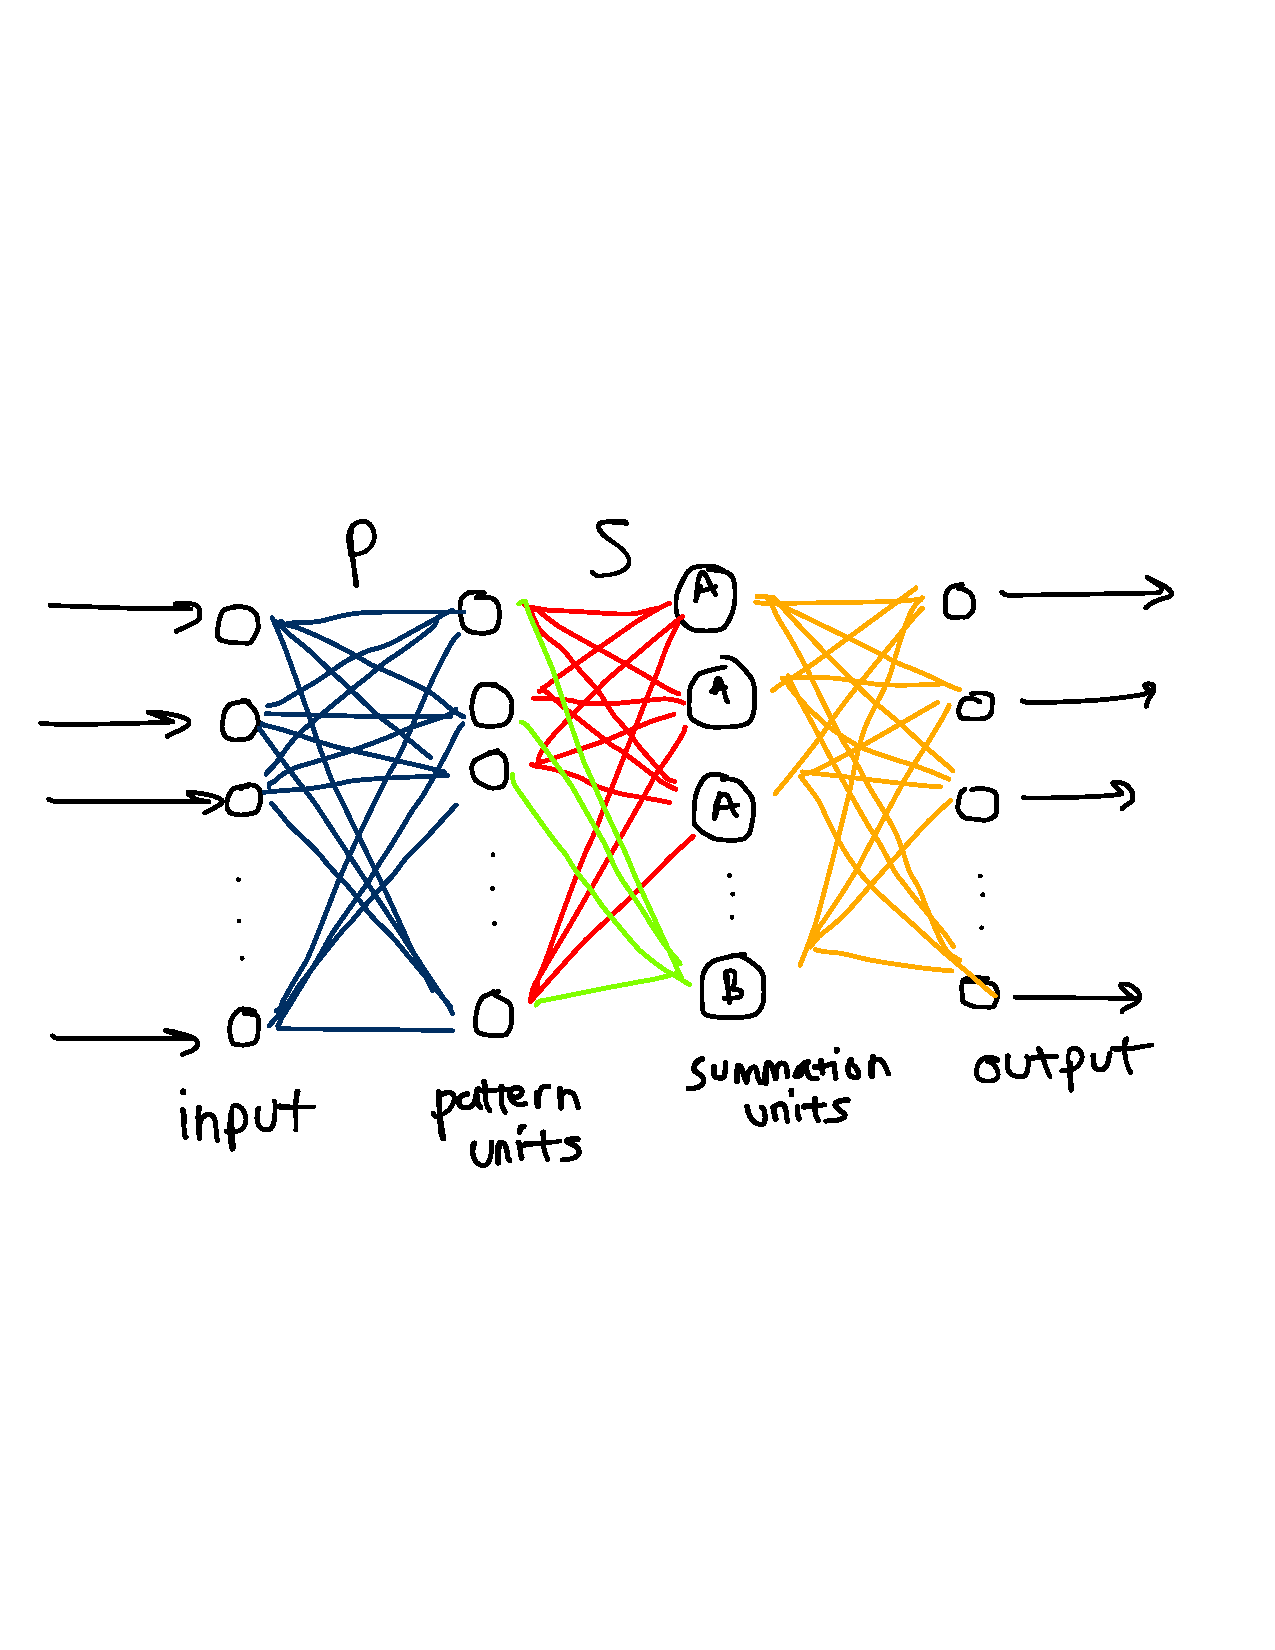
\includegraphics[width=0.48\textwidth]{../figures/GRNN-2.pdf}
  \label{fig:GRNN}
  \caption{The network as we drew it up. The weights between the input and pattern units are the matrix $P$, the weights between the pattern units and the summation units in red are the matrix $S$. The green weights between the pattern and summation units, and the orange weights between the summation units and output are all set to 1. I was also told that this looked like a bad football play diagram.}
\end{figure}

\begin{figure}
 \centering
  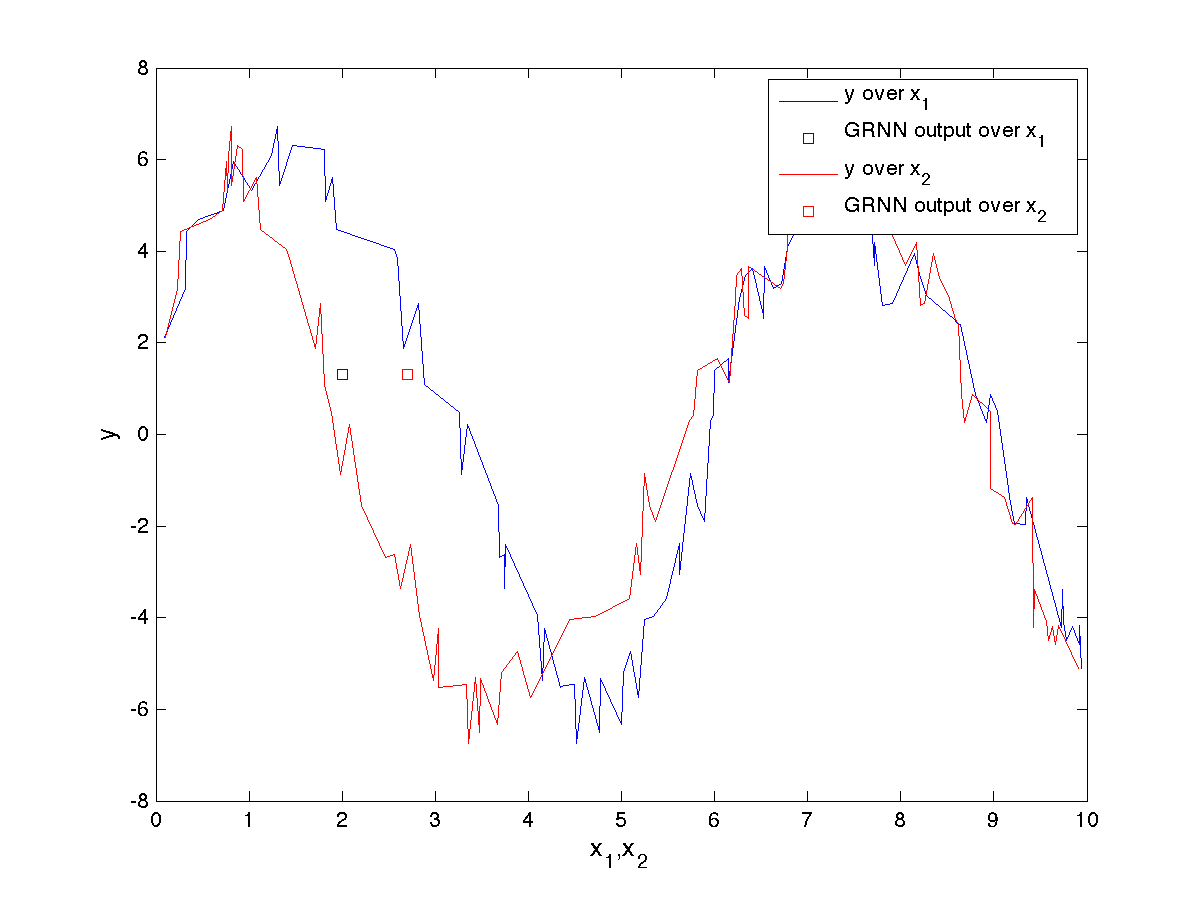
\includegraphics[width=0.48\textwidth]{../figures/GRNN.png}
  \label{fig:1}
  \caption{Interpolation of a single data point from very noisy data, $y$, from two inputs $x_1$ and $x_2$.}
\end{figure}

\section{Methods}

The network is coded as we drew it in class, see Figure 1.
Define the input patterns $X$ as a matrix with the patterns as rows, and $Y$ as the output patterns, with the outputs as rows.
In testing, I use a 2-D input pattern and a 1-D output.
As Specht notes in his paper, to generate additional output, another $A$ and $B$ unit are added for each output.

The weight matrix $P$ is simply the input patterns, and the non-unity weights $S$ are simply the output patterns.
So, we have that $P = X$ and $S = Y$, the other weights all being 1.
Tne only other piece is the activation function, which we write as
\begin{equation} f_\sigma(x) = \exp \left( \frac{x}{2\sigma} \right). \end{equation}

I generate some testing data by randomly pulling vectors in 2D for the $X$ input, and using a $\sin()$ function and noise for the output, making something that is not linear.
The $X$ patterns are both sampled from $[0,10]$ randomly, and then sorted.
The $Y$ output has uniform noise from $[0,1]$ added, and a in total is the function:
\begin{equation} Y = 3*\sin(X_1) + 3*\sin(X_2+1) + \mu. \end{equation}

In addition, I test the given testing data which looks like a sigmoidal function, and show the output curves for varying smoothing $\sigma$ in Figure 4.

\begin{figure}
 \centering
  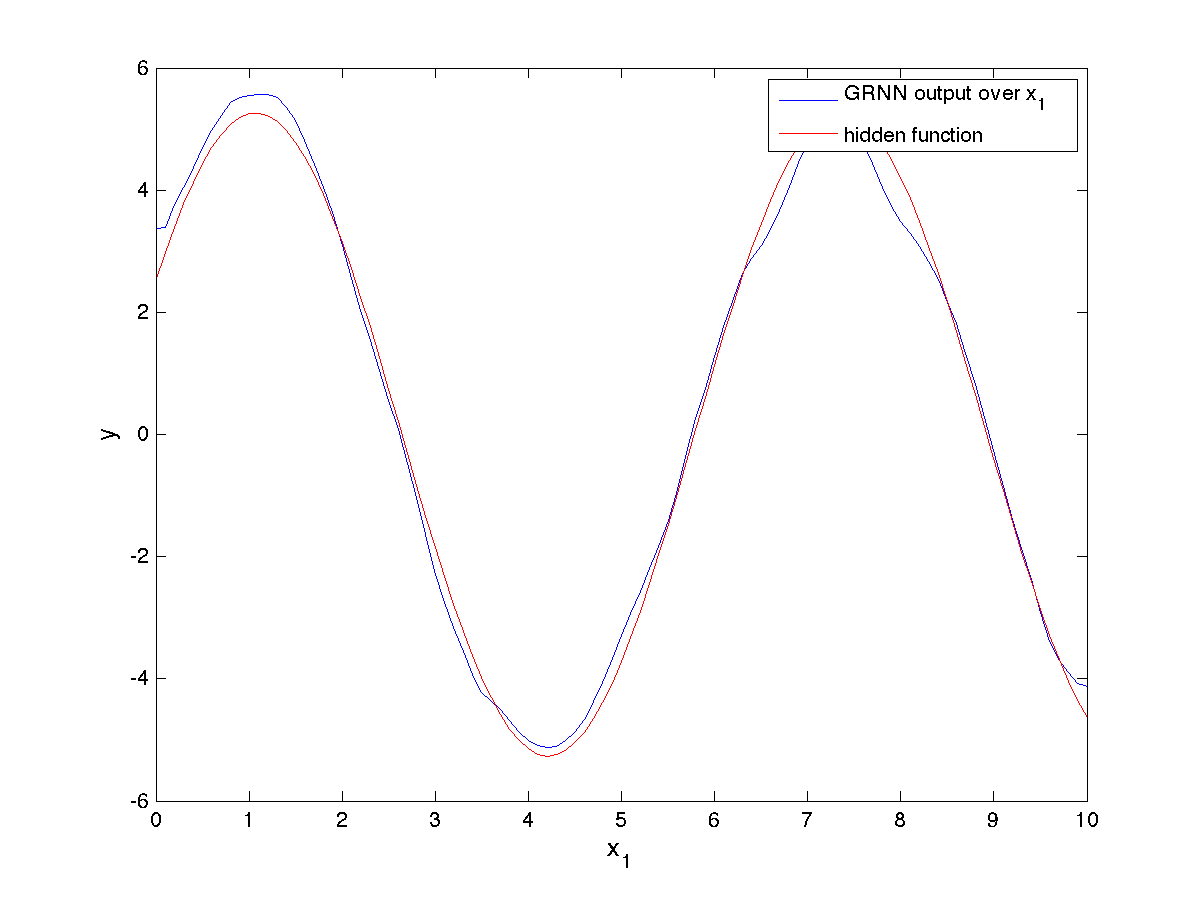
\includegraphics[width=0.48\textwidth]{../figures/GRNN-allx.png}
  \label{fig:2}
  \caption{Interpolation of $y$ using linearly spaced points over $x_1$ by the GRNN. The true function, hidden by uniform random noise of magnitude 1, is also shown.}
\end{figure}

\begin{figure}
 \centering
  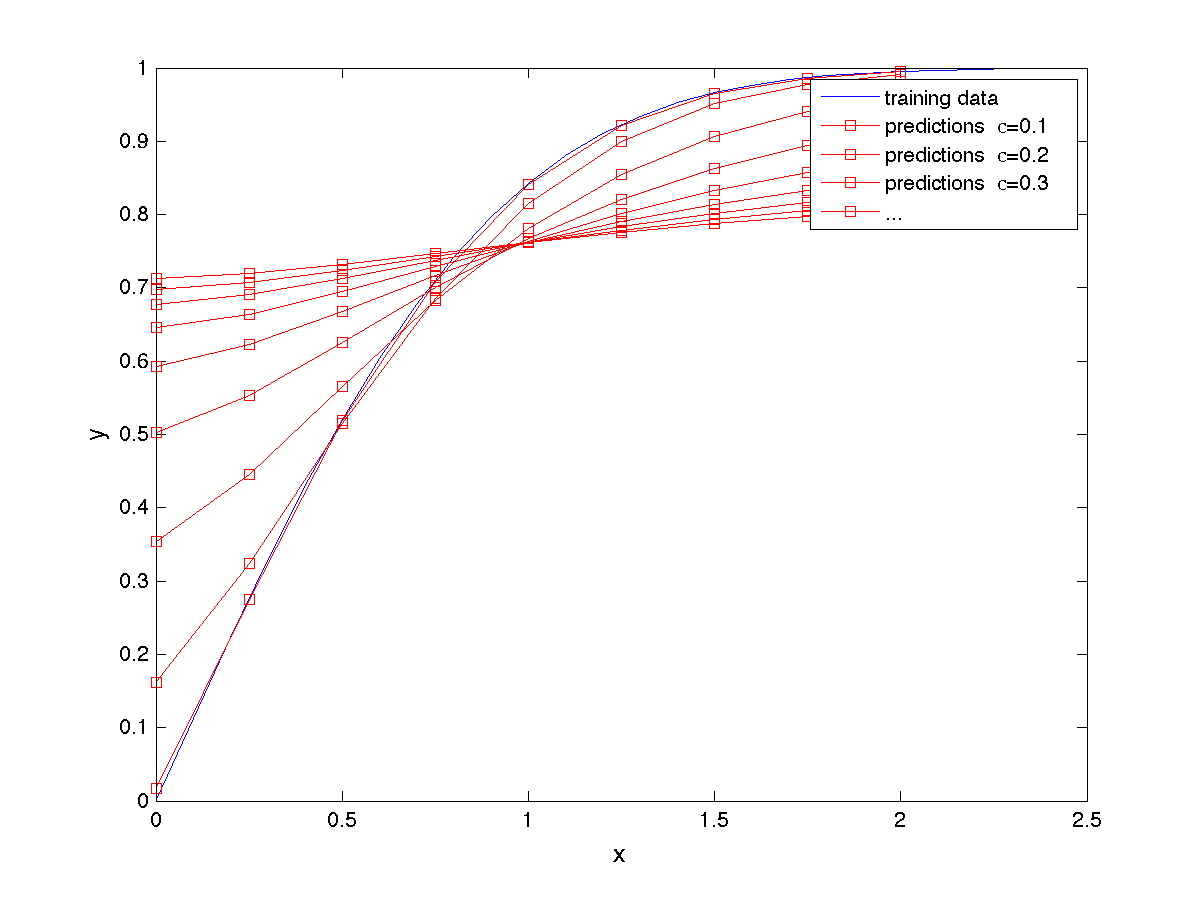
\includegraphics[width=0.48\textwidth]{../figures/GRNN-givenData-allsigma.png}
  \label{fig:3}
  \caption{Interpolation of sigmoid $y$ using linearly spaced points over $x_1$ by the GRNN. Both the training data (blue, no squares) and the GRNN interpolation for various $\sigma$ are plotted.}
\end{figure}

\begin{figure}
 \centering
  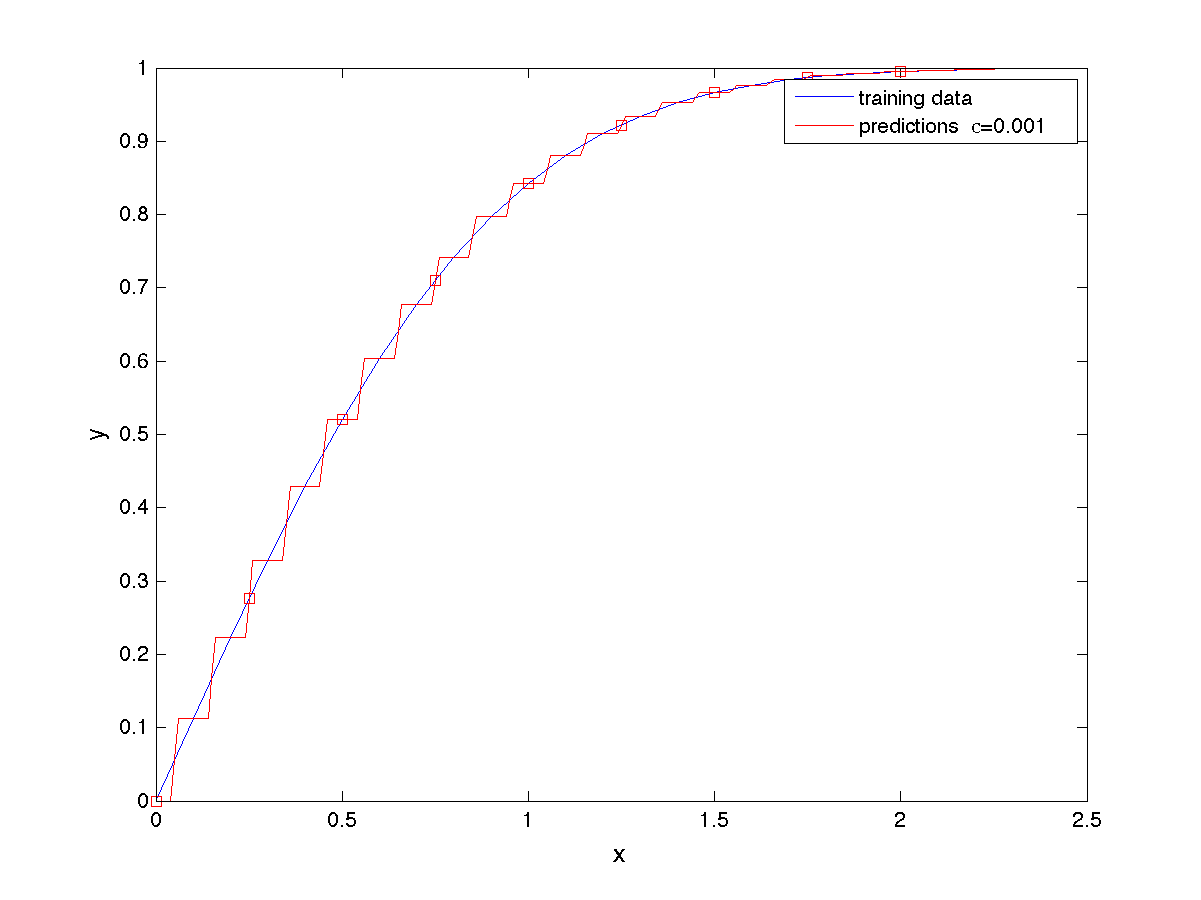
\includegraphics[width=0.48\textwidth]{../figures/GRNN-givenData-sigma0-001-sqdiff.png}
  \label{fig:4}
  \caption{Overfit of the GRNN.}
\end{figure}

\begin{figure}
 \centering
  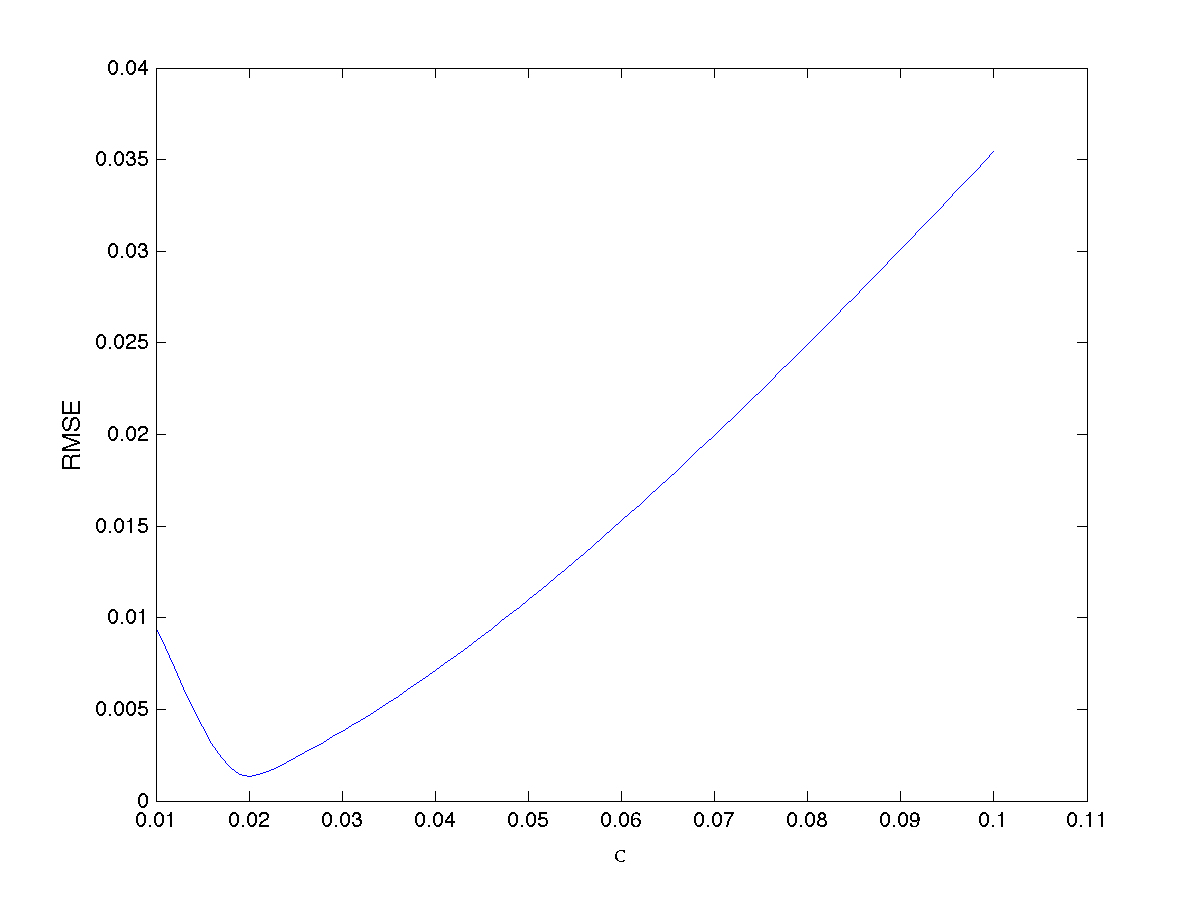
\includegraphics[width=0.48\textwidth]{../figures/GRNN-givenData-allsigma-sqdiff-RMSE-correct.png}
  \label{fig:5}
  \caption{RMSE versus the $\sigma$ parameter.}
\end{figure}

\section{Results}

A simple test of the network, and the coding of the network itself, demonstrate how easy it is to use.
In Figure 3, we see that it does a reasonably good job at approximating our nonlinear function, considering the substantial amount of noise that was applied.

To test the network was a little bit tricky, I had to use the trained GRNN to test against a smoothed version of the function, interpolated at the values.
In the end, I wrote my own $Y$ data, so I could generate a better, exact, interpolated dataset to test against.
The error that I showed you after class was me plotting the data wrong, I was plotting the transpose, oops!
Anyway, as $\sigma$ decreases we find a better and better approximation in Figure 4.

When $\sigma$ is sufficiently cranked down, the GRNN performs well.
It seems to me that $\sigma$ must be chosen to be a ``good bit'' smaller than the gaps between the training dataaset, to properly smooth.
When it is too big, the GRNN finds the mean of the data.
However, for very small $\sigma$, we do find an increase in the error as the GRNN overfits the data.
An example of what the overfit looks like is shown in Figure 5.

Finally, I plotted the RMSE over different $\sigma$ in Figure 6, and the GRNN does have an optimal value, as I hoped!
Without knowing the true function, I do think that the ``smaller than training gap'' rule of thumb would do okay, and just looking at the output for flat spots.

I wonder if symbolic regression could find this function from the given data.
Symbolic regression feels like a completely different solution to a very related problem, when the model is not known.
Fun!

\bibliographystyle{chicago}
\bibliography{writeup}

\clearpage
\pagebreak
\onecolumngrid

    \section*{Full code}

    \lstinputlisting{../GRNN_andy_driver.m}
    \lstinputlisting{../makeTrainingData.m}
    \lstinputlisting{../f.m}

%% \clearpage
%% \pagebreak

%%     \section*{Extra figures}

%%     %% \begin{figure}
%%     %%   \centering
%%     %%   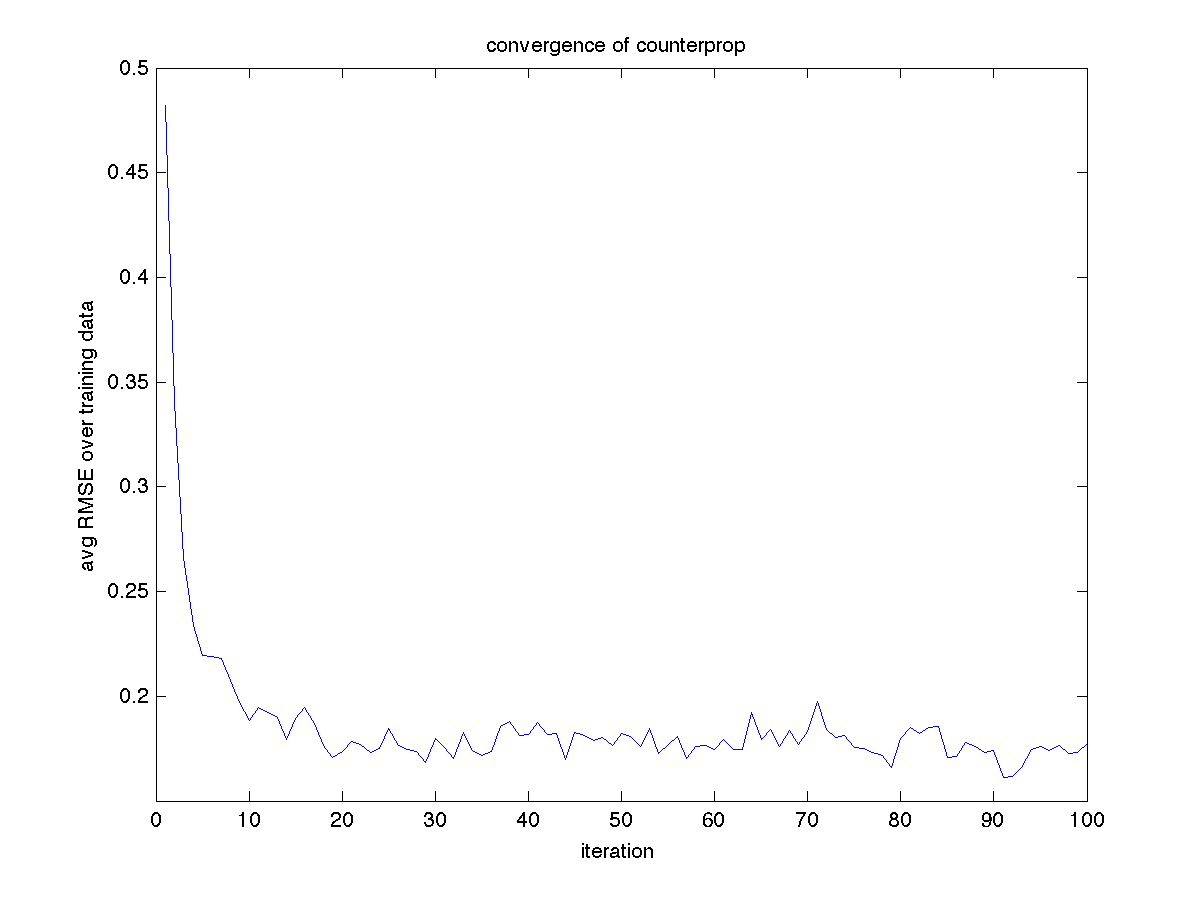
\includegraphics[width=0.68\textwidth]{111.png}
%%     %%   \label{fig:1}
%%     %%   \caption{Basic convergence test.}
%%     %% \end{figure}

\end{document}
